%! Author = matteomagnini
%! Date = 05/03/25

%----------------------------------------------------------------------------------------
\chapter[Platform for symbolic knowledge injection]{\Glsentrylong{PSyKI}}
\label{ch:psyki}
\minitoc
%----------------------------------------------------------------------------------------

In this chapter, we present the \Gls{PSyKI} platform, which is a framework for \gls{SKI} methods.
%
\Gls{PSyKI} provides a unified way to implement \gls{SKI} methods, aiming to facilitate the development and comparison of different approaches.
%
It also provides a set of tools to evaluate the performance of \gls{SKI} methods, including metrics for measuring the quality of the injected knowledge and the performance of the resulting models.
%
In \Cref{sec:psyki}, we present the work ``\emph{On the Design of PSyKI: A Platform for Symbolic Knowledge Injection into Sub-symbolic Predictors}''~\cite{DBLP:conf/atal/MagniniCO22}, which describes the design and implementation of \gls{PSyKI}.
%
Then, in \Cref{sec:qos}, we present respectively two works that study the quality of service of \gls{SKI} methods:
%
in \Cref{sec:ski-meets-intelligent-agents} the paper ``\emph{Symbolic Knowledge Injection Meets Intelligent Agents}''~\cite{DBLP:journals/aamas/AgiolloRMCO23},
%
which introduces metrics for evaluating the performance of \gls{SKI} methods in the context of intelligent agents,
%
and in \Cref{sec:empirical-study-on-the-robustness-of-ski-methods} the paper ``\emph{An Empirical Study on the Robustness of Symbolic Knowledge Injection Techniques Against Data Degradation}''~\cite{DBLP:conf/woa/RafanelliMACO24},
%
which studies the robustness of \gls{SKI} methods against data degradation.


\section{PSyKI}\label{sec:psyki}
%
\Gls{PSyKI} is a (Python) platform for the development and evaluation of \gls{SKI} methods.
%
It is designed to provide a unified framework for implementing \gls{SKI} methods, allowing researchers and practitioners to easily develop, test, and compare different approaches.
%
In the following, we present a summary of the work ``\emph{On the Design of PSyKI: A Platform for Symbolic Knowledge Injection into Sub-symbolic Predictors}''~\cite{DBLP:conf/atal/MagniniCO22}, presented at the 4th International Workshop on EXplainable, Trustworthy, and Responsible AI and Multi-Agent Systems (EXTRAAMAS 2022)\footnote{\url{https://extraamas.ehealth.hevs.ch/archive.html}}.
%
The library is public available on GitLab and PyPi\footnote{\url{https://gitlab.com/psykei/psyki-python} and \url{https://pypi.org/project/psyki/}}.


\subsection{Motivations}\label{subsec:psyki-motivations}
%
This work is motivated by the need to address the common challenges that affect \gls{SKI} methods (see \Cref{subsec:limitations-and-challenges-of-ski}).
%
In particular, we want to address the following points:
%
\begin{inlinelist}
    \item \emph{lack of generality}, by providing the proper tools to automatically translate symbolic knowledge of arbitrary domains into a format suitable for injection into sub-symbolic predictors,
    %
    \item \emph{lack of reproducibility}, by providing a unified framework for implementing \gls{SKI} methods, allowing researchers to easily develop, test, and compare different approaches, and
    %
    \item \emph{lack of availability}, by encouraging the development of reusable software libraries for \gls{SKI} methods.
    %
\end{inlinelist}
%
Concerning the last point mentioned in \Cref{subsec:limitations-and-challenges-of-ski}, we identified in the logic language of stratified Datalog with negation a suitable candidate for the symbolic knowledge representation.
%
It is expressive enough to represent a wide range of symbolic knowledge, while being simple enough to be easily translated into a format suitable for injection into sub-symbolic predictors.


\subsection{Design}\label{subsec:design-and-implementation}
%
\begin{figure}
    \centering
    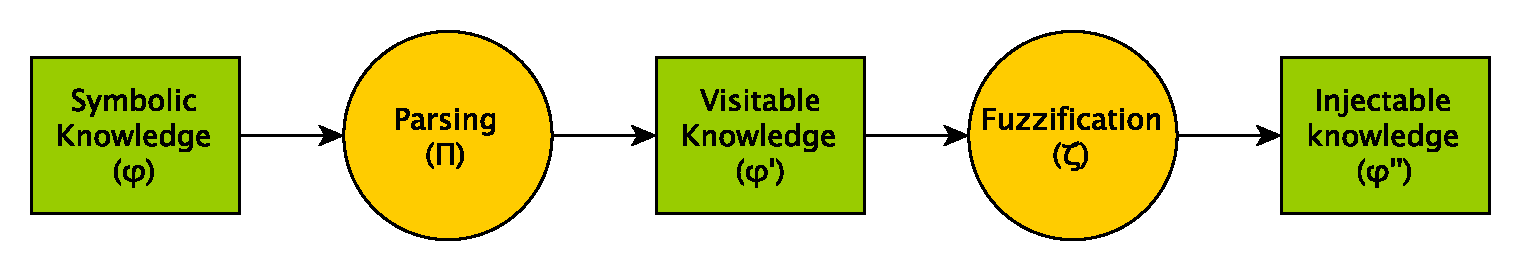
\includegraphics[width=\textwidth]{figures/knowledge-workflow-psyki}
    \caption[Symbolic knowledge transformation in PSyKI]{
        General workflow of symbolic knowledge transformation in \Gls{PSyKI}.
        The symbolic knowledge ($\phi$), typically expressed as logical formulas, is first parsed into a visitable form ($\phi'$), and then fuzzified into a machine-injectable representation ($\phi''$).
    }
    \label{fig:knowledge-workflow-psyki}
\end{figure}
%
All symbolic knowledge injection (\gls{SKI}) methods implemented in \gls{PSyKI} share a common transformation pipeline, illustrated in \Cref{fig:knowledge-workflow-psyki}.
%
Symbolic knowledge \(\phi\) cannot usually be injected directly into a sub-symbolic predictor.
%
Instead, it undergoes a two-step transformation:
%
\begin{inlinelist}
    %
    \item \emph{Parsing} (\(\Pi\)): the knowledge is converted into a visitable data structure, such as an \gls{AST} in the case of logic formulas, resulting in \(\phi'\);
    %
    \item \emph{Fuzzification} (\(\zeta\)): the parsed representation is transformed into a sub-symbolic form \(\phi''\), suitable for injection.
    %
\end{inlinelist}
%
Fuzzification plays a key role in bridging the symbolic and sub-symbolic domains.
%
It translates crisp Boolean logic into a form compatible with sub-symbolic models, often by relaxing discrete truth values into continuous-valued functions or generating neural components such as layers or entire \glspl{NN}.

\begin{figure}
    \centering
    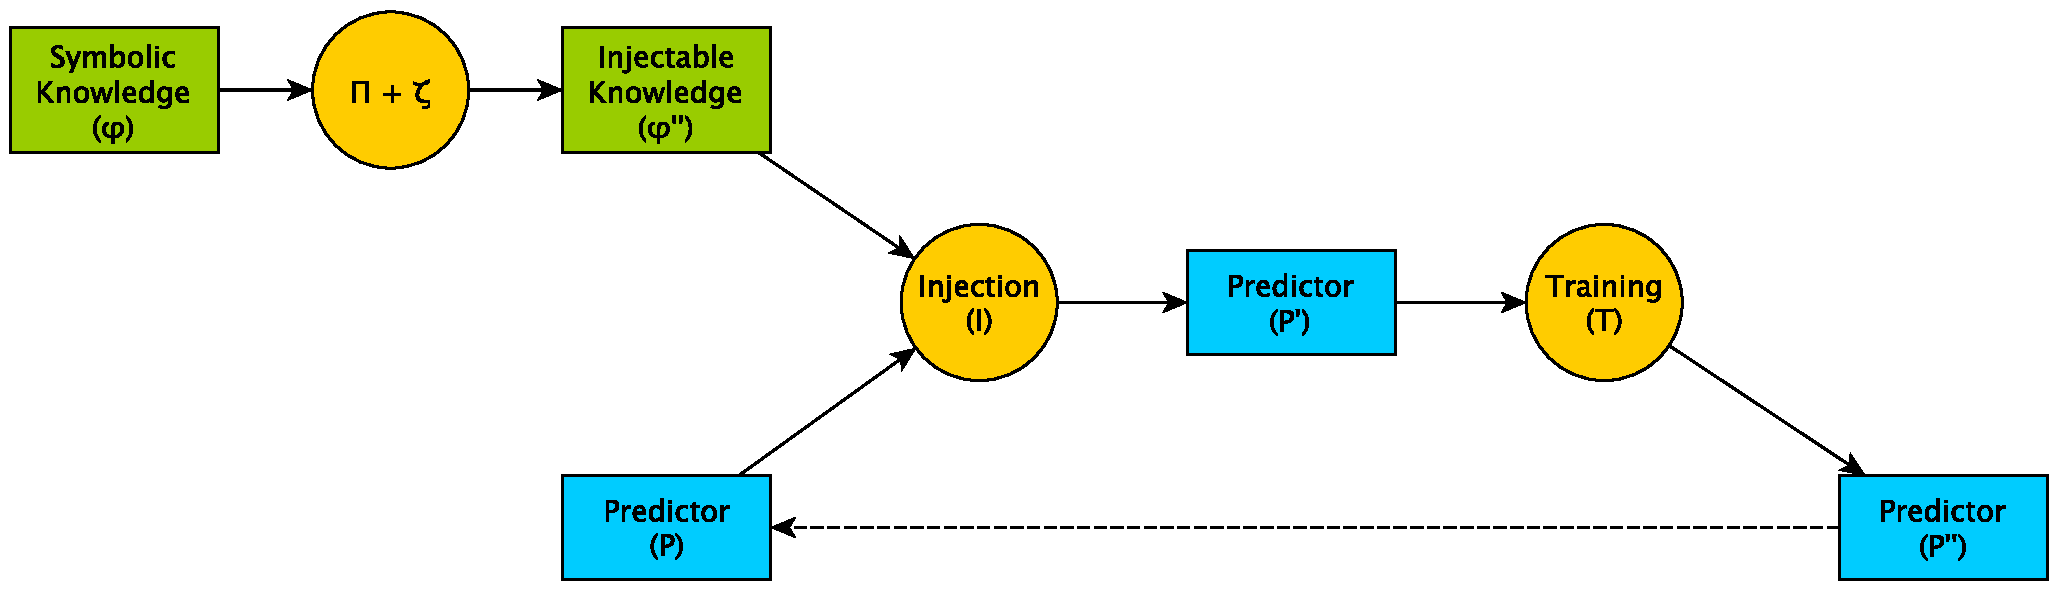
\includegraphics[width=\textwidth]{figures/psyki-workflow}
    \caption[General workflow of PSyKI]{
        Complete workflow of structuring and guided learning \gls{SKI} methods in \Gls{PSyKI}.
        The symbolic knowledge is transformed and injected into the sub-symbolic predictor, which is then trained on data.
    }
    \label{fig:psyki-workflow}
\end{figure}
%
\Cref{fig:psyki-workflow} shows the overall injection process in \gls{PSyKI}, including both the transformation of the symbolic knowledge and its integration into the learning system.
%
After the transformation phase, the different \gls{SKI} methods diverge:
%
\begin{inlinelist}
    %
    \item \emph{Structuring} and \emph{guided learning} inject \(\phi''\) directly into the architecture or training process of the predictor;
    %
    \item \emph{Embedding}-based methods use symbolic knowledge to enrich or generate the input data, so they are not directly represented in \Cref{fig:psyki-workflow}.
    %
\end{inlinelist}

\Gls{PSyKI} supports all three approaches, although it is primarily designed for \emph{structuring} and \emph{guided learning}, where the injection occurs directly into the predictor.
%
In general, \gls{SKI} algorithms operate on a predictor \(P\) and symbolic knowledge \(\phi\), producing a new predictor \(P'\) as output.
%
This modified predictor is then trained on data, resulting in a final model \(P''\), which can be reused in further iterations with different knowledge or injection strategies.


\paragraph{Architecture}\label{par:architecture}
%
\begin{figure}
    \centering
    \includegraphics[width=\textwidth]{figures/class-diagram}
    \caption[Class diagram of PSyKI]{
        Class diagram of \Gls{PSyKI}.
        %
        The main components are the \emph{Injector}, the \emph{Formula} and the \emph{Fuzzifier}.
        %
        The package \emph{logic.datalog} is an examplification showing two \emph{Injector} implementations and their relationships.
    }
    \label{fig:psyki-class-diagram}
\end{figure}
%
Essentially, \gls{PSyKI} is designed around the notion of injector.
%
An injector is any algorithm accepting a \gls{ML} predictor and prior symbolic knowledge -- predominantly logic formulas -- as input that produces a new predictor as output.
%
In order to properly perform injection, injectors may require additional information such as algorithm specific hyperparameters.


\gls{PSyKI} supports the processing of symbolic knowledge represented via logic formulas.
%
Based on the sort of logic, user can build an \gls{AST} for each formula.
%
The \gls{AST} can be inspected through a fuzzifier via pattern visitor to encode the symbolic knowledge to a sub-symbolic form (e.g. fuzzy logic functions, ad-hoc layers).
%
The resulting sub-symbolic object can finally be used by an injector to create a new predictor.
%
This process -- denoted with $\zeta$ \Cref{fig:psyki-workflow} -- is injector specific; instead, the same parser $\Pi$ can be used for logic formulas of the same sort independently of the injector.


The software is organized into well-separated packages to ensure easy extensibility towards new sort of logic and fuzzifiers---see \Cref{fig:psyki-class-diagram}
%
An \gls{AST} is a \emph{formula} object, and it can have different language specific elements w.r.t. the logic form that is covered.
%
Each formula implementation is self-contained inside a standalone package so that if a user wants to add a new logic form it is sufficient to add its implementation in a new package.
%
Similarly, a fuzzifier object that targets a specific logic form can be added inside the same package of the logic, there can be any number of fuzzifiers for a given logic.


\subsection{Implementation}\label{subsec:psyki-implementation}
%
\paragraph{Knowledge representation}\label{par:knowledge-representation}
%
\begin{figure}
    \centering
    \includegraphics[width=\textwidth]{figures/grammar}
    \caption[Class diagram for the representation of Datalog formulas]{
        A supported grammar of \Gls{PSyKI} for logic formulas.
        %
        The grammar is designed to represent Datalog formulas.
    }
    \label{fig:grammar}
\end{figure}
%
A crucial point in the \gls{SKI} workflow is the embedding of knowledge from symbolic into sub-symbolic form.
%
Ideally, there is no constraint on the formalism used to represent the prior knowledge (e.g., logic formulas, knowledge graph).
%
The most common knowledge representation form that \gls{SKI} algorithms claim to support is \gls{FOL} or one of its subsets.
%
However, there are characteristics of \gls{FOL} that are not ideal for some predictors.
%
Recursion and function symbols -- that allow recursive structures -- cannot be easily integrated into a predictor that is acyclic -- i.e., no recursive -- by construction such as conventional \gls{NN} (virtually all \gls{NN}, with few exceptions like fibred \gls{NN}~\cite{DBLP:conf/flairs/BaderGH05}).
%
Conversely, in this work we consider one of the most general and expressive logic formalism that does not support recursion and function symbols: stratified Datalog with negation.


Stratified Datalog with negation has been already described in detail in \Cref{subsec:ski-stratified-datalog-with-negation}.
%
To support injection into a particular predictor, we further assume the input knowledge base defines at least one outer relation -- say output or class -- involving as many variables as the input and output features the predictor has been trained upon.
%
Such a relation may be defined via one or more clauses, and each clause may leverage on other predicates in their bodies.
%
In turn, each predicate may be defined through one or more clause.
%
In that case, since we rely on stratified Datalog, we require input knowledge to not include any (directly or indirectly) recursive clause definition.


Once that the logic has been formalized, the implementation of a \emph{Formula} -- visitable data structure like an \gls{AST} -- is quite straightforward.
%
\Cref{fig:grammar} depicts the general API for representing logic formulas, as currently supported by \gls{PSyKI}.
%
To make \gls{PSyKI} able to parse bare text into actual logic formulas compliant to that API, we rely on well-established parser-generation facilities such as ANTLR~\cite{DBLP:journals/spe/ParrQ95}.
%
As further discussed below, the knowledge contained into a Formula object, can then be embedded in sub-symbolic form, via a fuzzifier, to be later injected into a predictor.


Later in the evolution of \gls{PSyKI} (i.e., from v. 0.2.1), we considered switching to a more established logic language for representing the symbolic knowledge: Prolog~\cite{DBLP:journals/tplp/KornerLBCDHMWDA22}.
%
In particular, we abandoned the manual parsing of logic formulas with ANTLR, and we rely on the tuProlog~\cite{DBLP:conf/padl/DentiOR01} framework.
%
We use the parser of tuProlog to parse the logic formulas, but \gls{PSyKI} does not support the full Prolog language because of the limitations of injecting into \gls{NN} mentioned in \Cref{subsec:limitations-and-challenges-of-ski} (i.e., we still support only stratified Datalog with negation).


\paragraph{Fuzzification}\label{par:fuzzification}
%
While logic formulas are commonly interpreted in a Boolean way -- i.e., they can be assigned with one truth value among true and false --, sub-symbolic predictors are more flexible-hence supporting formulas to hold up to some extent.
%
Switching from the former interpretation to the latter is, essentially, the purpose of fuzzifiers.
%
In practice, this implies converting a logic formula into a function of real numbers.
%
Along this line, fuzzification may be performed in (at least) two ways; real numbers may either represent
%
\begin{inlinelist}
    %
    \item a \emph{penalty} for the violation of a formula, or
    %
    \item the \emph{degree of truth} of that formula.
    %
\end{inlinelist}

To serve this purpose, one may rely on a multivalued interpretation of logic inspired to $\L$ukasiewicz's logic, where the value true is represented by 0 (resp. 1), while higher (resp. lower) values represent ``falsity''.
%
In particular, this approach may be useful to constrain a predictor during its training.
%
Examples of this fuzzification approach are \gls{KILL} (\Cref{subsec:kill-fuzzifier}) and \gls{KINS} (\Cref{subsec:kins-fuzzifier}).
%
\Cref{tab:kill-logic-formulae,tab:kins-logic-formulae} show the logic formulas encoding into real-valued functions for \gls{KILL} and \gls{KINS}, implementing \emph{penalty} and \emph{degree of truth} respectively.


\paragraph{Injection}\label{par:injection}
%
\lstinputlisting[
    basicstyle=\fontsize{8}{9.5}\ttfamily\selectfont,
    label=lst:psyki-injection,
    float,
    caption={General code snippet for the use of a \gls{SKI} method in the current version of \gls{PSyKI} (v. 0.4.3).},
    captionpos=b,
    language=Python,
]{listings/psyki-injection.py}
%
Knowledge injection is the central step in \gls{SKI}.
%
It is carried out by \emph{injectors}, i.e., objects wrapping a particular injection strategy.
%
Each injector is expected to accept one sub-symbolic predictors as input, other the logic formulas that should be injected into that predictor.
%
As part of its operation, the injector is in charge of producing a new predictor as output, of the same type as the one provided as input.
%
The new predictor is altered in such a way that it is consistent w.r.t. the provided logic formulas.


While the main architecture of \gls{PSyKI} has been maintained stable during the years, the implementation has been continuously improved.
%
The current version of \gls{PSyKI} (v. 0.4.3) is implemented in Python 3.9.13, with main dependencies being \texttt{tensorflow}, \texttt{2ppy}, \texttt{scikit-learn}, and \texttt{pandas}.
%
\Cref{lst:psyki-injection} shows a general code snippet for the use of a \gls{SKI} algorithm in \gls{PSyKI} (v. 0.4.3).


\section[SKI meets intelligent agents]{\Gls{SKI} meets intelligent agents}\label{sec:ski-meets-intelligent-agents}
%
In this and in the next section, we present two works that study the \gls{QoS} of \gls{SKI} methods.
%
\Gls{QoS} is a crucial aspect of any non-trivial systems, and it is particularly important for \gls{SKI} because the vast majority of the works in this field do not provide any evaluation but the performance of the resulting model.
%
Moreover, \gls{SKI} methods and the resulting educated models have many other dimensions that can be evaluated a part from the straight prediction performance.
%
The metrics introduced in these works have been implemented and integrated into \gls{PSyKI} from version 0.2.14 and later.


The work ``\emph{Symbolic Knowledge Injection Meets Intelligent Agents}''~\cite{DBLP:journals/aamas/AgiolloRMCO23}, published in the \emph{Autonomous Agents and Multi-Agent Systems} journal, presents a set of metrics for evaluating the performance of \gls{SKI} methods in the context of intelligent agents.
%
Here we present a summary of the work, including the motivations, the proposed metrics, and the evaluation of \gls{SKI} methods in terms of \gls{QoS}.


\subsection{Motivations}\label{subsec:ski-meets-intelligent-agents-motivations}
%
The current practice of assessing \gls{SKI} methods primarily focuses on measuring improvements in the predictive performance of an educated predictor \(\hat{N}\) over its uneducated counterpart \(N\).
%
However, predictive performance is not the only relevant benefit of \gls{SKI} that should be evaluated.

There are multiple aspects of \glspl{ML} predictors that can be influenced by \gls{SKI}, and for which specific metrics should be defined.
%
For instance, \gls{SKI} may impact the \emph{memory footprint}, \emph{latency}, \emph{data efficiency}, and \emph{energy consumption} of the predictors it is applied to.
%
Collectively, these properties contribute to what we refer to as the \emph{efficiency} of a predictor.

In this work, we consider the following efficiency properties:
%
\begin{properties}
    \item \textbf{Memory footprint}: the size of the predictor, typically measured in terms of the number of parameters or computational operations required.
    %
    \label{itm:memory-footprint}
    %
    \item \textbf{Latency}: the time required to perform a single inference.
    %
    \label{itm:latency}
    %
    \item \textbf{Data efficiency}: the amount of data required to train the predictor to achieve a certain level of performance.
    %
    \label{itm:data-efficiency}
    %
    \item \textbf{Energy consumption}: the energy required to train and/or run the predictor.
    %
    \label{itm:energy-consumption}
    %
    \item \textbf{Predictive performance}: standard metrics such as accuracy, F1-score, or mean squared error.
    %
    \label{itm:predictive-performance}
\end{properties}

For brevity, we refer to any function that measures one of these properties as an \emph{efficiency metric}.
%
These metrics quantify the improvement in a given property \(P\) of the uneducated predictor \(N\) when transformed into its educated counterpart \(\hat{N}\) through a \gls{SKI} mechanism.

The resulting efficiency scores can be influenced by several factors:
%
\begin{factors}
    %
    \item \textbf{Knowledge quality and coverage}:
    %
    The educated predictor \(\hat{N}\) is obtained by injecting symbolic knowledge \(K\).
    %
    Both \(N\) and \(\hat{N}\) are trained on the same dataset \(D\), which describes the learning task.
    %
    Key questions include:
    %
    \begin{inlinelist}
        \item Are \(K\) and \(D\) coherent?
        \item Does \(K\) cover situations exemplified in \(D\)?
        \item Is \(K\) consistent, coherent, and correct?
        \item Can the same be said for \(D\)?
    \end{inlinelist}
    %
    The answers to these questions significantly affect the efficiency scores, as they depend on the interplay between \(K\) and \(D\).
    %
    \label{itm:knowledge-quality-and-coverage}

    \item \textbf{Baseline quality}:
    %
    Both \(N\) and \(\hat{N}\) target the same learning task.
    %
    Questions to consider include:
    %
    \begin{inlinelist}
        \item Is \(N\) biased in a statistical sense?
        \item If so, can \(\hat{N}\) improve any efficiency metric \(P\)?
        \item Even if \(N\) is unbiased, is the selected injection mechanism \(\mathcal{I}\) suitable for \(N\)?
    \end{inlinelist}
    %
    These factors highlight the dependency of efficiency measures on the nature of \(N\) and the injection mechanism \(\mathcal{I}\).
    %
    \label{itm:baseline-quality}

    \item \textbf{Task at hand}:
    %
    The learning task determines the training dataset \(D\) and the test dataset \(T\).
    %
    The choice of \(T\) impacts the evaluation of both \(N\) and \(\hat{N}\), and consequently, the efficiency scores.
    %
    \label{itm:task-at-hand}
\end{factors}

In summary, efficiency metrics evaluate a \gls{SKI} method \(\mathcal{I}\) in a specific context defined by:
%
\begin{inlinelist}
    \item the symbolic knowledge \(K\),
    \item the predictor \(N\),
    \item the training dataset \(D\), and
    \item the test dataset \(T\).
\end{inlinelist}
%
Thus, any efficiency metric must be parametric with respect to \(K\), \(N\), \(D\), and \(T\).


\subsection{Metrics}\label{subsec:ski-meets-intelligent-agents-metrics}
%
In this section, we propose the implementation and formalization of metrics to evaluate the efficiency of \gls{SKI} methods.
%
Specifically, we introduce \emph{memory footprint}, \emph{latency}, \emph{energy consumption}, and \emph{data efficiency} as key performance indicators for assessing \gls{SKI}.
%
These metrics aim to quantify the computational resource usage of \gls{SKI} methods and provide insights into their design and optimization.
%
Our focus is on understanding how these metrics can guide the development of \gls{SKI}-based systems, particularly within the context of \glspl{MAS}.
%
An in-depth analysis of the trade-offs between performance and efficiency is crucial for the effective implementation of AI predictors in \glspl{MAS}.
%

\subsubsection{Memory footprint}\label{subsubsec:ski-meets-intelligent-agents-memory-footprint}
%
In the context of \glspl{MAS}, the importance of sub-symbolic predictors is growing as the field moves towards more efficient and sustainable \gls{AI}.
%
The increasing demand for \gls{AI} systems that can operate on resource-constrained devices, such as IoT and edge devices, has driven research into solutions requiring less memory and computational resources~\cite{CITATION}.
%
Several metrics have been proposed to measure the memory footprint of \gls{AI} predictors, particularly sub-symbolic ones~\cite{CITATION}.
%
For instance, the memory footprint of \glspl{NN} can be quantified by counting their parameters, \glspl{FLOP}, or \glspl{MAC}, which represent the operations required for a single inference~\cite{CITATION}.
%
These metrics are effective for analyzing predictor complexity and computational efficiency.

%
\Gls{SKI} mechanisms can reduce the memory footprint of sub-symbolic predictors by injecting prior knowledge, thereby reducing the need for data-driven learning of complex concepts.
%
This reduction in learned concepts often translates to fewer parameters, \glspl{FLOP}, and \glspl{MAC}, resulting in a smaller memory footprint~\cite{CITATION}.
%
We define the memory footprint improvement score as the memory saved by the educated predictor \(\hat{N}\) compared to its uneducated counterpart \(N\):
%
\begin{equation}
    \label{eq:memory-footprint-improvement-score}
    \mu_{\Psi, K, N}(\mathcal{I}) = \Psi(N) - \Psi(\mathcal{I}(K, N)),
\end{equation}
%
where \(\mathcal{I}(K, N)\) (a.k.a., $\hat{N}$) represents the educated predictor obtained by injecting symbolic knowledge \(K\) into \(N\).

%
The improvement score depends on the quality and coverage of the input knowledge (\Cref{itm:knowledge-quality-and-coverage}) and the memory footprint of the input predictor (\Cref{itm:baseline-quality}).
%
Higher-quality knowledge reduces the memory requirements of the educated predictor.
%
Similarly, predictors with lower initial memory footprints exhibit smaller improvements.
%
It is important to note that the memory footprint of a \gls{NN} is task-independent, as it is a structural property of the network.

%
Finally, a negative score indicates that the educated predictor is more memory-intensive than the uneducated one, suggesting that the \gls{SKI} approach is ineffective in reducing memory usage.


\subsubsection{Energy consumption}\label{subsubsec:ski-meets-intelligent-agents-energy-consumption}
%
The relationship between \glspl{MAS} and energy consumption is multifaceted and critical.
%
To operate effectively in resource-constrained environments, \glspl{MAS} require \gls{AI} systems that minimize energy usage.
%
The distributed nature of \glspl{MAS}, combined with the increasing demand for scalable and power-efficient solutions, further emphasizes this need.
%
However, the dynamic and real-time requirements of many \glspl{MAS} applications often lead to high energy consumption due to computational and resource demands.
%
The complexity of \glspl{MAS}, with multiple agents and their interactions, adds another layer of difficulty, especially when processing large datasets or executing complex algorithms.
%
Thus, energy consumption becomes a crucial factor in the design and implementation of \gls{AI} systems within \glspl{MAS}~\cite{CITATION}.

%
Several strategies can address this challenge.
%
One approach involves using energy-efficient hardware, such as low-power processors, or adopting distributed and federated learning techniques to distribute computational loads across multiple devices~\cite{CITATION}.
%
Another approach focuses on optimizing algorithms and data structures to reduce the computational requirements of agents.
%
The integration of sub-symbolic predictors, which typically require fewer computational resources than symbolic \gls{AI} methods, can also significantly reduce energy consumption.
%
Additionally, techniques such as compression and optimization of sub-symbolic predictors can further enhance energy efficiency~\cite{CITATION}.

%
\gls{SKI} methods offer a promising opportunity to improve energy efficiency in \glspl{MAS}.
%
By introducing injection mechanisms into the data-driven pipeline of sub-symbolic training, \gls{SKI} reduces the computational complexity of training and running predictors.
%
This is achieved by leveraging prior knowledge, which complements the training data and simplifies the learning process.
%
As a result, it is essential to evaluate the extent to which \gls{SKI} mechanisms contribute to reducing the energy consumption of sub-symbolic predictors throughout their lifecycle.

%
To analyze energy consumption, we first define the lifecycle of \gls{AI} predictors, which includes the following stages:
%
\begin{enumerate}
    \item \textbf{Model definition}: Data scientists analyze the task and select suitable sub-symbolic predictors and hyperparameters.
    %
    \item \textbf{Model training}: The predictor's parameters are tuned using training data, where the size and dimensionality of the dataset impact energy consumption.
    %
    \item \textbf{Model testing}: The predictor is evaluated on a limited test set to ensure satisfactory performance.
    %
    \item \textbf{Model deployment}: The predictor is used for inference, with energy consumption depending on usage frequency and application lifespan.
\end{enumerate}

%
Among these stages, training and deployment are the most resource-intensive.
%
Training involves repeated executions and updates of the predictor, while deployment energy consumption depends on the frequency and duration of usage, which are often unpredictable.

%
We propose two metrics to measure energy consumption:
%
\begin{itemize}
    \item \textbf{Inference energy consumption}:
    %
    The average energy consumed by a predictor \(N\) for a single inference is defined as:
    %
    \begin{equation}
        \label{eq:inference-energy}
        \Upsilon^\mathsf{i}_{\upsilon}(N, T) = \frac{1}{\vert T \vert} \sum_{t \in T} \upsilon(N, t),
    \end{equation}
    %
    where \(\upsilon(N, t)\) measures the energy consumed by \(N\) during inference on a sample \(t\) from the test set \(T\).
    %
    \item \textbf{Training energy consumption}:
    %
    The average energy consumed during training is defined as:
    %
    \begin{equation}
        \label{eq:training-energy}
        \Upsilon^\mathsf{t}_{\upsilon, \gamma}(e, N, T) = \frac{\gamma(e, N, T)}{e \cdot \vert T \vert} -  \Upsilon^\mathsf{i}_\upsilon(N, T),
    \end{equation}
    %
    where \(e\) is the number of epochs, \(|T|\) is the size of the training set, and \(\gamma(e, N, T)\) estimates the total energy consumed during training, including inference costs.
\end{itemize}

%
The energy consumption improvement of a \gls{SKI} mechanism \(\mathcal{I}\) is defined as the energy saved by the educated predictor \(\hat{N} = \mathcal{I}(K, N)\) compared to the uneducated predictor \(N\).
%
We distinguish between improvements during inference and training:
%
\begin{align}
    \varepsilon^\mathsf{i}_{\upsilon, K, N, T}(\mathcal{I}) &= \Upsilon^\mathsf{i}_{\upsilon}(N, T) - \Upsilon^\mathsf{i}_{\upsilon}(\mathcal{I}(K, N), T)
    \\
    \varepsilon^\mathsf{t}_{\upsilon, \gamma, e, K, N, T}(\mathcal{I}) &= \Upsilon^\mathsf{t}_{\upsilon, \gamma}(e, N, T) - \Upsilon^\mathsf{t}_{\upsilon, \gamma}(e, \mathcal{I}(K, N), T)
\end{align}

%
These metrics depend on several factors:
%
\begin{itemize}
    \item \textbf{Input knowledge (\Cref{itm:knowledge-quality-and-coverage})}: Complex knowledge may increase training energy consumption but reduce inference energy.
    %
    \item \textbf{Baseline predictor (\Cref{itm:baseline-quality})}: Energy-hungry predictors are more likely to benefit from \gls{SKI}.
    %
    \item \textbf{Task at hand (\Cref{itm:task-at-hand})}: Task-specific datasets influence energy consumption improvements.
\end{itemize}

%
In summary, \gls{SKI} mechanisms have the potential to significantly reduce energy consumption in \glspl{MAS}, particularly during inference, while potentially increasing training energy costs.
%
These trade-offs must be carefully evaluated to optimize the overall efficiency of \gls{AI} systems.


\subsubsection{Latency}\label{subsubsec:ski-meets-intelligent-agents-latency}
%
Latency refers to the time required to generate a single prediction using a sub-symbolic predictor.
%
Low latency is crucial in real-world applications where timely responses are essential, such as in intelligent transportation~\cite{CITATION} and e-health~\cite{CITATION}.
%
In \glspl{MAS}, latency plays a significant role as collaboration between agents requires minimal computational delays~\cite{CITATION}.
%
Additionally, tasks involving large datasets or complex algorithms, such as decision-making, can further increase latency, making it a critical efficiency measure.

%
\gls{SKI} methods can help reduce latency by incorporating symbolic representations, which simplify computations and reduce the complexity of the system.
%
This simplification can also aid in identifying the root causes of increased latency, making \gls{SKI} a valuable approach for improving computational efficiency.

%
Latency is typically measured as the average time required to generate predictions over a test dataset \(T\).
%
Formally, the latency of a predictor \(N\) is defined as:
%
\begin{equation}
    \label{eq:latency}
    \Lambda(N, T) = \frac{1}{\vert T \vert} \sum_{t \in T} \Theta(N, t),
\end{equation}
%
where \(\Theta(N, t)\) represents the time taken by \(N\) to generate a prediction for a sample \(t \in T\).

%
To evaluate the impact of \gls{SKI}, we define the latency gain $\lambda_{K, N, T}(\mathcal{I})$ as the difference in latency between the educated predictor \(\hat{N} = \mathcal{I}(K, N)\) and the uneducated predictor \(N\):
%
\begin{equation}
    \label{eq:latency-gain}
    \lambda_{K, N, T}(\mathcal{I}) = \frac{1}{\vert T \vert} \sum_{t \in T} \left( \Theta(N, t) - \Theta(\hat{N}, t) \right) = \Lambda(N, T) - \Lambda(\hat{N}, T),
\end{equation}
%
where \(\mathcal{I}(K, N)\) represents the \gls{SKI} mechanism injecting symbolic knowledge \(K\) into \(N\).

%
The latency gain depends on several factors:
%
\begin{itemize}
    \item \textbf{Input knowledge (\Cref{itm:knowledge-quality-and-coverage})}: Large or complex knowledge bases may increase latency due to additional computations, but they can also reduce inference time by simplifying the predictor's operations.
    %
    \item \textbf{Baseline predictor (\Cref{itm:baseline-quality})}: Predictors with higher initial latency are more likely to benefit from \gls{SKI}.
    %
    \item \textbf{Task at hand (\Cref{itm:task-at-hand})}: Task-specific datasets influence latency measurements, as different tasks may require varying levels of computational effort.
\end{itemize}

%
It is important to note that latency is not always directly proportional to the number of operations in the predictor.
%
Sparse or inefficient operations at the hardware level, as well as variations in input data complexity, can significantly affect latency~\cite{CITATION}.
%
Thus, evaluating latency gain provides valuable insights into the computational efficiency of \gls{SKI} methods.


\subsubsection{Data efficiency}\label{subsubsec:ski-meets-intelligent-agents-data-efficiency}
%
Data-efficiency is a critical aspect of \glspl{MAS}, as these systems often generate and process substantial amounts of data.
%
Inefficient data management can lead to increased latency, reduced accuracy, and higher energy consumption, all of which negatively impact system performance.

%
Sub-symbolic predictors, which rely on data-driven training algorithms, offer significant flexibility and performance.
%
However, they require large amounts of data for training, resulting in increased storage and processing demands.
%
Moreover, the quality of the data, particularly its representativeness of the task, is crucial for effective learning.
%
These requirements make data collection time-consuming and potentially prone to subjectivity or uncertainty, as seen in applications like emotion recognition~\cite{CITATION}.

%
Recent research has focused on developing data-frugal predictors~\cite{CITATION}.
%
Among these, \gls{SKI} mechanisms play a significant role by leveraging \emph{a priori} knowledge to reduce the computational burden of learning.
%
Instead of learning all concepts from data, \gls{SKI} allows injecting prior knowledge into the predictor, potentially reducing the amount of data required to achieve acceptable performance levels.
%
In this sense, \gls{SKI} can be considered a data-efficiency mechanism.

%
To quantify the data-efficiency gain of a given \gls{SKI} mechanism \(\mathcal{I}\), we first define the \emph{data footprint} of a predictor \(N\).
%
The data footprint represents the amount of data required to train \(N\) to achieve a specific performance level.
%
Assuming \(N\) is trained on a dataset \(D\) with samples of varying dimensions, over \(e\) epochs, and achieves a performance score \(\pi(N, T)\) on a test set \(T\), the data footprint is defined as:
%
\begin{equation}
    \label{eq:data-footprint}
    \Delta_\pi(e, N, D, T) = \frac{e}{\pi(N, T)} \sum_{d \in D} \beta(d),
\end{equation}
%
where \(\beta(d)\) is the memory size (in bytes) of a single training sample \(d\).

%
The data-efficiency gain of a \gls{SKI} mechanism \(\mathcal{I}\) is then defined as the difference between the data footprints of the uneducated predictor \(N\) and the educated predictor \(\hat{N} = \mathcal{I}(K, N)\), trained on datasets \(D\) and \(D'\), respectively:
%
\begin{equation}
    \label{eq:data-efficiency-gain}
    \delta_{e, K, N, D, D', T}(\mathcal{I}) = \Delta_\pi(e, N, D, T) - \Delta_\pi(e, \mathcal{I}(K, N), D', T)
\end{equation}

%
To improve data-efficiency, one can reduce the size of the training dataset \(D'\), either by decreasing the number of samples or by reducing their dimensionality through compression.
%
Additionally, engineering the \gls{SKI} mechanism and the educated predictor can further enhance data-efficiency.
%
For instance, the input knowledge \(K\) can compensate for the reduced dataset size, as the gain depends on both the quality of \(K\) (\Cref{itm:knowledge-quality-and-coverage}) and the baseline predictor (\Cref{itm:baseline-quality}).
%
Predictors that are more data-hungry tend to exhibit higher data-efficiency gains.


\section[Empirical study on the robustness of SKI methods]{Empirical study on the robustness of \Gls{SKI} methods}\label{sec:empirical-study-on-the-robustness-of-ski-methods}
%
\note{TODO: present the paper An Empirical Study on the Robustness of Symbolic Knowledge Injection Techniques Against Data Degradation~\cite{DBLP:conf/woa/RafanelliMACO24}}
